\documentclass[a4paper,11pt]{article}
\usepackage[a4paper, includefoot]{geometry}
\usepackage[parfill]{parskip}
\usepackage{ctable}
\usepackage{url}
\usepackage{graphicx}
\usepackage{paralist}
\usepackage{verbatim}

\begin{document}
\title{WebApps Group Project: Project Report} \date{12th June
  2013} \author{
  Thai Tam Nguyen $<$ttn211@imperial.ac.uk$>$\\
  Jo Schlemper $<$js3611@imperial.ac.uk$>$\\
  Terence Tse  $<$tt1611@imperial.ac.uk$>$ }
\maketitle
%\newpage

Where is my money App.
\section*{Introduction (10\% Aim for half a page?)}

Requirement:
An app used by people in a shared environment, such as a flat or a university, to keep track of debts.
Requirement \& target
Target: 
An app which supports people living together?  

\section*{Project Management (30\% Aim for 1 ~ 1.5 pages)}
Group Structure:\\
Group Leader: \\
Jo Schlemper\\
Group members: \\
Thai tam Nguyen \\
Terence Tse\\
Implementation Language:\\
Client Side: Android \\
Server Side: Java + Tomcat\\
Database: Postgresql\\
Design process:\\
Feedback from the team members. \\
Classic approach. Design on a paper? Dunno what to write here. \\
Back-ups:\\
GitHub \\

\section*{Program (40\% Aim for 6 pages with pictures)}
\subsection*{Description}
Our final product is an android application which keeps track of debts. Once a user registers to the database, the user can create new transactions, view transactions and confirm the payment or the partial payment for transactions. The application provides the ability to make transactions to an individual or a group. It also supports messaging for individuals or a group, which can be used as a mean to communicate with each other, urge one another to pay and so on. The view of the transactions can be customised according to the users’ preference: per person or per item. Per person displays a list of people who you owe or who owes you and total amount of the debt. Clicking on the entry allows you to view a profile page, from which you can nudge, message, call and make a new transaction to the person. It also provides a log of transactions you have with the person.

\subsection*{Design Patterns}
Although the fundamental idea of the application is fairly simple, achieving the functionalities require careful considerations of design patterns. 

\subsubsection*{Classic 3-tier architecture}
For multiple users to interact with one another, it is necessary to have a convention for the communication of data. To achieve this we decided to deploy a classic 3-tier architecture as having a database on the server simplifies this communication process. Every time when a user requests to view or create transactions, the requests will be sent to the server through HTTP methods, GET or POST. For our application, it is unnecessary to serve a page; instead, we pass around a data between the client and the server in JSON format. The reason why we chose JSON is because it is a standard format for passing data through networks. It means that there are many third party libraries for encoding and decoding JSON string. For the client side, we used the standard library from Android to decode JSON string; on the client side, we wrote a code which builds a JSON string. 

\begin{figure}[ht]
\begin{center}
\advance\leftskip-3cm
\advance\rightskip-3cm
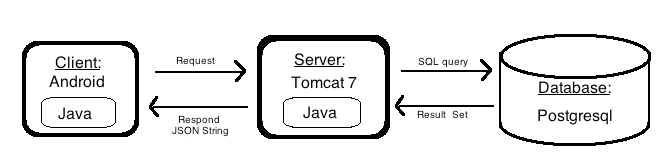
\includegraphics[keepaspectratio=true,scale=0.5]{3tier}
\caption{The 3-tier Architecutre}
\label{visina8}
\end{center}
\end{figure}

\subsubsection*{Builder pattern}
To build a JSON string from the server side, we wrote a class \texttt{JSONBuilder.java} which lets you to build a JSON string. JSON string requires specific characters such as `$\lbrace$' `:' and writing the string manually could be erroneous so using the builder not only lets you make use of the pattern, it also simplifies the code and yet relatively easier to read. 

\begin{verbatim}
//... execute SQL query and obtain a set of results in transactionSet
// Build JSON string
JSONBuilder jb = new JSONBuilder();
jb.beginObject().append("returnCode",1).beginArray();
while (transactionSet.next()) {
//...Obtain the result
						
jb.beginObject().append("transid", transId)
                .append("name",transName)
                .append("total_amount",transAmount)
  .endObject();
}
jb.endArray().endObject();			
writer.println(jb.build());
\end{verbatim}

\subsubsection*{Singleton}
HttpClient as a singleton pattern. Use 

\subsubsection*{Concurrency}
 Future and AsyncTask
 
\subsubsection*{Observer Pattern}
onClickListener for listView 
 
\subsubsection*{Template Method}
CustomAdopter for list view.

\subsubsection*{General Style}
Encapsulation

 
\section{Acknowledgement (doesn’t count, keep minimum)}
Android SDK? Not sure if needed to mention here though.
CustomHttpClient.java from Android Developers: http://developerrohit.blogspot.co.uk/2011/04/customhttpclientjava.html
Took as an inspiration for our client side HTTP methods such as GET and POST.
We created our own logo and icons so we should not have any problem for copyright. 
\section*{Conclusion (20\% 1~1.5pages including acknowledgement)}

We all love octopussy.\\


BELOW HERE WHAT YOU WROTE BEFORE\\


\section*{Preface}
While sharing a flat with some friends, naturally, we decided to pool together money and share payments for things such as groceries, meals out and utility bills. Everyone who shares a flat knows the troubles associated with tracking payment to your friends, and even more so, chasing them down for your money. Our group intends to develop and application which will allow such situations to be resolved easily. This will be targeted, ideally, at students who are sharing a flat. Of course, we do not intend to restrict the application to this group - the application could be loosely used to help simply track debts in between friends, for example when they go out, share a meal and have one person foot the bill.

\section*{Group arrangement}
Although we shall all be helping one another in every aspect of the project, we found it to be a good idea to split the problem into 3 main parts for each of us to "take charge" of. If one part gets finished before the others, then of course we will collbaorate to finish the remaining bits.\\ 
Thai Tam shall be managing the app GUI and the general graphical representation and visual aspects of the application.\\
Jo shall be in charge of the core of the application such as how to link the database to the application and how different sections of the application interact with one another and the database and web server.\\
Terence shall be in charge of managing the database and its updates as well as its maintenance and any other general issues that they may involve.

\section*{Implementation Language}

After a short discussion, we decided to develop an application for Android phones. One reason for this was that to develop for android you need to use Java which is the programming language we are, collectively, most proficient in. Choosing to develop an iOS application requires knowledge, or learning, of Objective-C and this could detract us from more interesting options, such as extending the application. Furthermore, there are many existing templates for android applications which will save us time in the design stage of the project as we can draw inspiration from the templates. \\
We have also decided to design for mobile devices as it would be more flexible than having the software situated on the web, while still allowing us the possibility of adding a web version of the application at a later date.

\section*{The Idea}

\subsection*{Application Basics}
The main focus of the application is to keep track of money that is owed to the user as well as the amount that he owes to other friends. All users will have an account when using this application, which will allow them to link with each other. If an involved person does not have the app, it will serve as a stripped down version of the app, resembling a memo.

The debt tracking part of the application can be thought of in two modes: a per item mode or a per person mode. The user can switch between these two modes within the settings of the application.  
Additional parts of the application we thought of which greatly extend its functionality and motivation for use include a messaging system, a calendar and 'wish lists' for the time being. 

'Reminders' in the app act as the 'Where's my money?' question we want to yell at our friends all too much. We all feel a little awkward pestering each other to return money so this app does it for you!
The reminders will be automatic or user incurred. Every time the user opens up the application, they will be reminded of any outstanding debts to pay. Since that may not be enough, we also decided to allow users to send reminders to others that money is due to be paid, manually. 

\subsubsection*{Per Item Mode}
We consider a 'transaction' or some form of payment as an 'item'. Thus, transactions of money in real life will be logged in a database and presented to the user on screen. It shall be displayed as a 'log' in a chronological list format. 
A transaction will hold the following pieces of data about it:
\begin{itemize}
\item{Date created}
\item{Transaction name (a short note about what the payment concerns)}
\item{Total sum of money to be collected}
\item{Person(s) involved in the transaction}
\item{Extra notes, a section for user input}
\end{itemize}
The idea is to have the list display just the core details: transaction name, persons involved (or a somewhat cut off list) and the debt amount. The user can then look up further information about the transaction by simply selecting the entry in the log. A new window displaying the information shall then pop up. When a transaction concerns multiple people, the extended information will show the user how much each person of the group owes as a portion of the total.
The log shall be displayed in chronological order but may be edited slightly based on urgency of payment collection. This will be useful for emergency situations, such as when you need the money for a utility bill, or simply because the person who owes you is leaving the country for an extended period.

\subsubsection*{Per Person Mode}
Per person mode differs from the per item mode by its 'contact list'-type log, where every person you have entered into the application will have an monetary value affiliated with their name. This value will be the overall total amount you owe to or are owed by that person as a result of the agglomerated transactions. 
We found that this is a very useful and actually quite popular method of keeping track of the debt between friends; people will usually keep track of the overall amount they owe each other, in absence of an application like ours. For example, I owed Jo \pounds5, I might have paid for the next meal which equated to \pounds7 and thus he'd just pay me \pounds2. 
The rest of this mode shall follow suit of the per item mode. When you click on a person you shall get a new pop up window, or 'profile' page, which will show you a log of all the transactions between you and the person you have selected.

\subsection*{User Interaction}
Obviously, to add a new transaction into the database of the app, the user has manually input data, i.e. the amount to be paid. The input method will be made as simple as possible. There will also be the option to form a 'group payment' involving multiple users for one transaction. There will also be an 'equal split' button which allows for quick calculation of how much each person owes as part of the bill if it were split evenly. This does not necessarily need to be used to hold the data as a transaction, but simply splitting a bill equally.

\subsubsection*{Messaging}
The messaging feature of this application was initially to supplement the 'reminders' that the application offers. For example, if someone kept bothering you with reminders but you had the valid reason that your pay check doesn't arrive until Friday, then a message could be sent to explain that.
We saw that this was necessary but we also realised it would be quite easy to extend this feature to emulate a fully fledged messenger application, such as group chats. This will allow communication for those transactions that involve multiple people, and therefore, whatever compromises they may reach, or insults they throw about, to be accommodated.

\subsubsection*{Calender}
The Calendar feature allows for a richening of the debt tracking feature. We intend to use this feature to add deadlines to payments which can then synthesize with our idea of an urgency rate on debts. The deadline feature can also collaborate with the reminders the app already provides.
There are other uses we are planning for this feature such as pinning events or things like utility bill deadlines.

\subsubsection*{Wish list}
The Wish List is a small trinket we all thought would be a nice addition to our application. In essence, it is a shared shopping list. A user may also conjoin lists with a friend who owns the app so that each may view the others' wish list. This means that if a certain flat member is out at the supermarket, they can check their conjoined lists and help buy things the other needs, in order to save multiple trips to the supermarket.
This will require the implementation of a synchronisation measure for these wish lists. The lists will need to update on all devices whenever someone adds to it. At the moment, we are proposing this update check takes place every time the user starts the application. However we are still contemplating this due to the overhead this will incur.

\end{document}
